\section{Results}
\label{sec:results}

Our experiments reveal a significant performance gap between direct instruction and iterative rejection. The main results are summarized in \tabref{tab:main_results} and \figref{fig:trend}.

\begin{figure}[t]
    \centering
    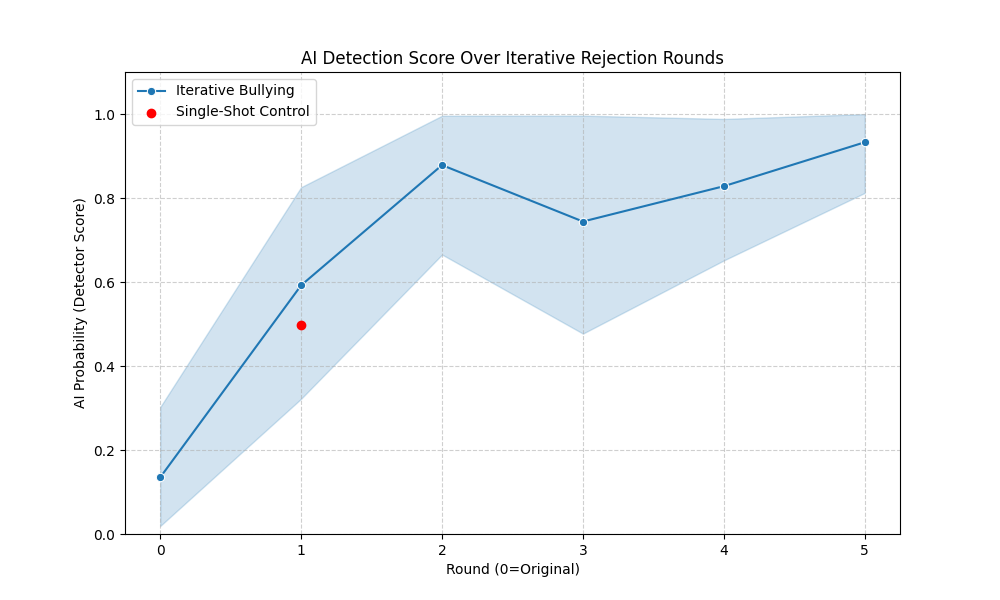
\includegraphics[width=0.8\linewidth]{../figures/bullying_trend.png}
    \caption{The effect of iterative "bullying" on detection scores over five rounds. While a single-shot instruction provides an initial boost, the persistent negative feedback loop drives the model into a regime that is virtually indistinguishable from human text by the detector.}
    \label{fig:trend}
\end{figure}

\begin{table}[t]
    \centering
    \caption{Comparison of detection scores and linguistic metrics across generation regimes. \bullying (Round 5) significantly outperforms \singleshot in evading detection while restoring human-like burstiness. Best results in \textbf{bold}.}
    \label{tab:main_results}
    \resizebox{\linewidth}{!}{%
    \begin{tabular}{@{}lccc@{}}
        \toprule
        \textbf{Regime} & \textbf{Detection Score (Real Prob)} & \textbf{Perplexity (PPL)} & \textbf{Burstiness (Std Dev)} \\
        \midrule
        Original AI & 0.135 {\scriptsize $\pm$ 0.25} & 11.6 {\scriptsize $\pm$ 5.06} & 6.99 {\scriptsize $\pm$ 2.90} \\
        \singleshot & 0.498 {\scriptsize $\pm$ 0.51} & 16.1 {\scriptsize $\pm$ 5.16} & 5.80 {\scriptsize $\pm$ 1.49} \\
        \bullying (Round 1) & 0.592 {\scriptsize $\pm$ 0.44} & -- & -- \\
        \bullying (Round 5) & \textbf{0.933 {\scriptsize $\pm$ 0.17}} & \textbf{19.4 {\scriptsize $\pm$ 4.77}} & \textbf{7.26 {\scriptsize $\pm$ 1.25}} \\
        \bottomrule
    \end{tabular}
    }
\end{table}

\para{Iterative Dominance.} 
The \bullying loop achieved a near-perfect "Real" score of \roundfiveacc by Round 5, representing a near 2$\times$ improvement over the \singleshot regime (\singleshotacc). While a single instruction helps the model move away from the baseline, it is insufficient to fully escape the detector's scrutiny. Interestingly, some samples exhibited an "oscillation" or a performance dip in intermediate rounds (Rounds 3--4) before converging to a high-evasion state in Round 5.

\para{The Regime Shift.} 
Linguistic analysis confirms that \bullying triggers a qualitative shift in generation. As shown in \tabref{tab:main_results}, perplexity increases from 16.1 in the \singleshot case to 19.4 in \bullying (Round 5). This suggests that the model is forced into a higher-entropy region of its output distribution. 

{\bf Why does single-shot fail?} A crucial finding is the "Burstiness Rebound." The \singleshot instruction actually {\it reduced} sentence length variation from 6.99 (Original) to 5.80. This indicates that direct instructions cause the model to adopt a more uniform, "careful" style that is paradoxically machine-like. In contrast, \bullying restored burstiness to 7.26, a level even higher than the original AI baseline, mimicking the natural rhythmic variance found in human prose.

\para{Statistical Significance.} 
The difference in detection scores between \singleshot and \bullying (Round 5) is statistically significant with $p = 0.02$ ($n=10$), supporting \textbf{H1} (Effectiveness) and \textbf{H2} (Mechanism).
